\documentclass[11pt]{beamer}
\usetheme{CambridgeUS}
\usepackage[utf8]{inputenc}
\usepackage{amsmath}
\usepackage{amsfonts}
\usepackage{amssymb}
\usepackage{graphicx}
\usepackage{pgfpages}
\usepackage{framed}
\usepackage{xcolor}
\usepackage[most]{tcolorbox}
\usepackage{soul}
\usepackage{empheq}

% The replacement character � (often displayed as a black rhombus with a white
% question mark) is a symbol found in the Unicode standard at code point U
% +FFFD in the Specials table. It is used to indicate problems when a system 
% is unable to render a stream of data to a correct symbol.[4] It is usually 
% seen when the data is invalid and does not match any character. For this 
% reason we map explicitly this character to a blanck space.
\DeclareUnicodeCharacter{FFFD}{ }

\newcommand*{\itemimg}[1]{%
  \raisebox{-.3\baselineskip}{%
    \includegraphics[
      height=\baselineskip,
      width=\baselineskip,
      keepaspectratio,
    ]{#1}%
  }%
}

\newtcbox{\mymath}[1][]{%
    nobeforeafter, math upper, tcbox raise base,
    enhanced, colframe=blue!30!black,
    colback=blue!10, boxrule=1pt,
    #1}

\newcommand{\hlym}[1]{%
  \colorbox{yellow!100}{$\displaystyle#1$}}

\newcommand{\hlgm}[1]{%
  \colorbox{green!100}{$\displaystyle#1$}}

\newcommand{\hly}[1]{\colorbox{yellow!100}{#1}}

\newcommand{\hlg}[1]{\colorbox{green!100}{#1}}

\author{Giovanni Della Lunga\\{\footnotesize giovanni.dellalunga@unibo.it}}
\title{1.1 - Introduction to Machine Learning}
%\title{1.2 - Data Gathering with Pandas}
%\title{2.1 - Data Pre-Processing}
%\title{4.1 - Linear and Logistic Regression}
%\title{4.2 - Decision Trees}
%\title{6 - Text Vectorization}
%\title{7 - Classification for Text Analysis}
%\title{8 - Clustering for Text Similarity}
%\title{9 - Information Extraction}
\subtitle{} % (optional)
\setbeamercovered{transparent} 
\institute{Introduction to Machine Learning for Finance} 
\date{Bologna - February-March, 2025} 

\begin{document}

%\begin{frame}
%\includegraphics[width=\linewidth]{img/halloween-seminar-logo.PNG}
%\end{frame}

\begin{frame}
\titlepage
\end{frame}

\AtBeginSection[]
{
  %\begin{frame}<beamer>
  %\footnotesize	
  %\frametitle{Outline}
  %\begin{multicols}{2}
  %\tableofcontents[currentsection]
  %\end{multicols}	  
  %\normalsize
  %\end{frame}
  \begin{frame}
  \vfill
  \centering
  \begin{beamercolorbox}[sep=8pt,center,shadow=true,rounded=true]{title}  	\usebeamerfont{title}\insertsectionhead\par%
  \end{beamercolorbox}
  \vfill
  \end{frame}
}
\AtBeginSubsection{\frame{\subsectionpage}}

% INSERT HERE
\begin{frame}{Introduction to Machine Learning for Finance}
\begin{itemize}
\item \textbf{Welcome to the Course!}
\vspace{.5cm}
\begin{itemize}
\item Instructor: Giovanni Della Lunga
\item Contact: giovanni.dellalunga@unibo.it
\item Course Duration: February-March 2025
\end{itemize}
\vspace{.5cm}
\item \textbf{Course Goals:}
\vspace{.5cm}
\begin{itemize}
\item Develop a solid understanding of Machine Learning (ML) fundamentals.
\item Explore ML applications in finance, including prediction and risk assessment.
\item Gain hands-on experience with Python tools for ML.
\end{itemize}
\end{itemize}
\end{frame}
%..................................................................
\begin{frame}{Introduction to Machine Learning for Finance}

\textbf{Lecture Overview}\\

In this lesson, we will explore the foundational concepts of Machine Learning (ML). \\

\textbf{Key Topics Covered}\\

\begin{itemize}
\item What is Machine Learning? Definitions and core principles.
\item Types of ML: Supervised, Unsupervised, Semi-supervised, and Reinforcement Learning.
\item ML workflow: Data gathering, preprocessing, modeling, and evaluation.
\item Essential ML concepts: Features, labels, cost functions, and optimization.
\item Introduction to Python tools for ML: Pandas, scikit-learn, and Jupyter Notebooks.
\item Using Pandas for financial data gathering.
\end{itemize}
\end{frame}
%..................................................................
\begin{frame}{Introduction to Machine Learning for Finance}

\textbf{Learning Objectives}
\vspace{1cm}
By the end of this lesson, students will:
\begin{itemize}
\item Understand the fundamental concepts of ML and its role in finance.
\item Recognize different types of ML models (Supervised, Unsupervised, etc.).
\item Learn how to gather and preprocess financial data using Python (Pandas, DataReader, yFinance).
\item Gain an overview of the ML workflow from data collection to model optimization.
\end{itemize}
\end{frame}
%===================================================================================================
\section{What is Machine Learning?
\\ \scalebox{0.8}{Basic Definitions}}
%---------------------------------------------------------------------------------------------------
\begin{frame}{Defining Machine Learning}
	\begin{itemize}
		\item Machine Learning is a scientific field within artificial intelligence (AI) that focuses on developing algorithms capable of learning from data. 

		\item These algorithms identify patterns, relationships, or recurring motifs in data, which can include numerical information, textual content, images, or statistical records. 

		\item Essentially, ML enables systems to perform tasks, make predictions, and improve their performance over time without explicit programming. 

		\item This process involves feeding data into algorithms that, through analysis, uncover underlying structures to predict outcomes, classify information, or group similar entities.

	\end{itemize}
\end{frame}
%..................................................................
\begin{frame}{Defining Machine Learning}
	Machine Learning is a process where a \textbf{Model} learns from \textbf{Data} to make predictions or decisions. It compares its predictions to the actual outcomes, calculating the \textbf{Error}. Then, through \textbf{Optimization}, the model adjusts itself to reduce this error and improve its performance over time.
	\begin{center}
	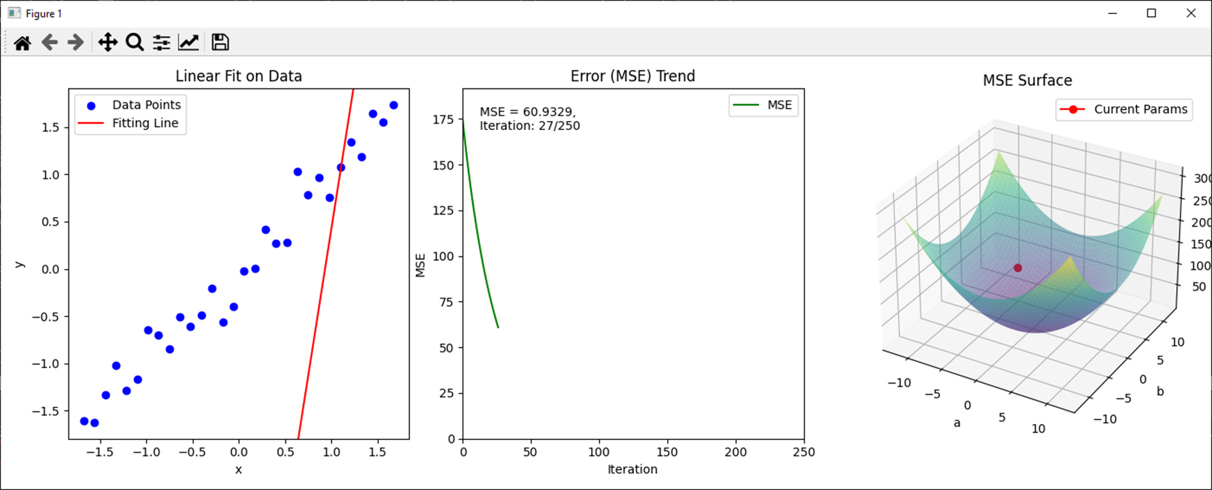
\includegraphics[scale=0.38]{../05-pictures/lesson-1-1_pic_0.png}
	\end{center}
\end{frame}
%..................................................................
\begin{frame}{Defining Machine Learning}
\footnotesize{\textbf{Data} are the foundation of machine learning, as models rely on it to identify patterns and make predictions. In a dataset, \textbf{features} are the input variables that describe the data, while \textbf{labels} are the target outputs the model aims to predict or classify. Features provide the information, and labels define what the model is learning to predict.}

	\begin{center}
	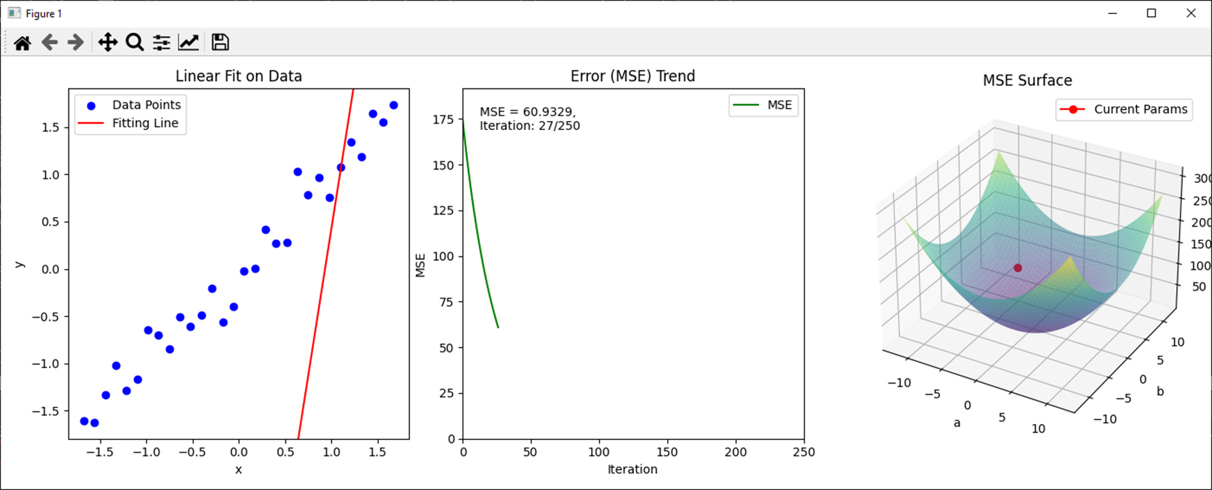
\includegraphics[scale=0.38]{../05-pictures/lesson-1-1_pic_1.png}
	\end{center}
\end{frame}
%..................................................................
\begin{frame}{Defining Machine Learning}
	\footnotesize{The \textbf{model} is the core of machine learning; it defines how data is processed to generate predictions. In simple linear regression, the model represents the relationship between input features and a target label as a straight line: $y = a + b*X$. Here, $b$ (slope) and $a$  (intercept) are parameters that the model learns from data. By adjusting these parameters during training, the model captures the underlying trend, enabling it to make accurate predictions on new data. } 
	\begin{center}
	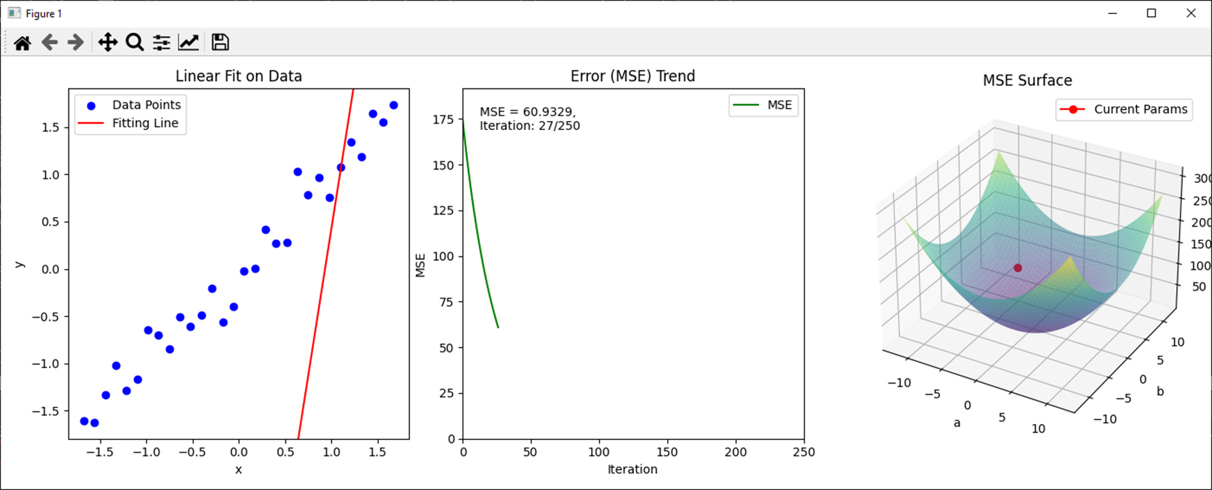
\includegraphics[scale=0.38]{../05-pictures/lesson-1-1_pic_2.png}
	\end{center}
\end{frame}
%..................................................................
\begin{frame}{Defining Machine Learning}
	\footnotesize{An \textbf{error measure} is essential in machine learning to quantify how far the model's predictions are from the actual values. It provides a way to evaluate the model's performance and guides improvements. By minimizing the error through optimization, we ensure the model learns effectively and generalizes well to new data. } 
	\begin{center}
	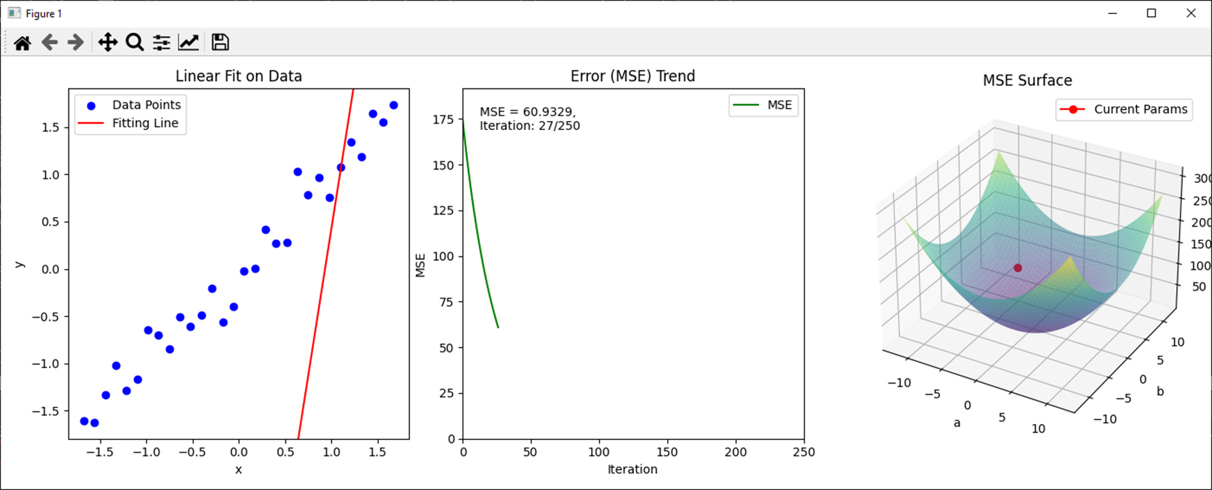
\includegraphics[scale=0.38]{../05-pictures/lesson-1-1_pic_3.png}
	\end{center}
\end{frame}
%..................................................................
\begin{frame}{Defining Machine Learning}
	\footnotesize{An \textbf{optimizer} is used to adjust the model's parameters (e.g., weights in linear regression) to minimize the error. It works by iteratively updating the parameters in the direction that reduces the error, typically using methods like gradient descent. The optimizer calculates the gradient of the error with respect to the parameters and updates them step by step, ensuring the model improves its predictions over time. } 
	\begin{center}
	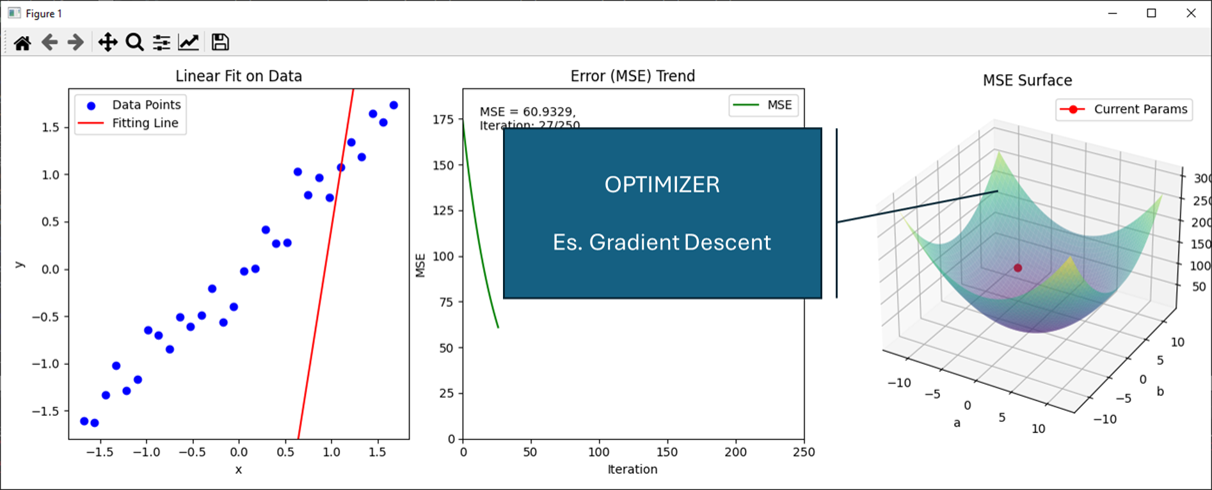
\includegraphics[scale=0.38]{../05-pictures/lesson-1-1_pic_4.png}
	\end{center}
\end{frame}
%..................................................................
\begin{frame}{Defining Machine Learning}
	Click the link below to play the video: \href{run:training-explication.mp4}{\textbf{Play Video}}
\end{frame}
%..................................................................
\begin{frame}{Defining Machine Learning}{Applications in Banking and Finance}
	Machine Learning finds applications across diverse fields.
	\begin{center}
	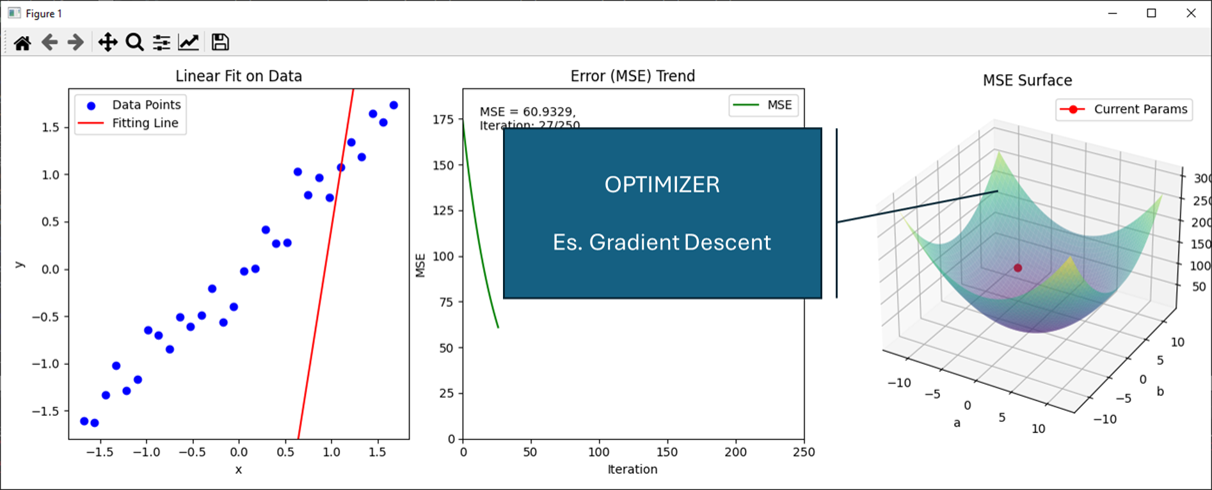
\includegraphics[scale=0.3]{../05-pictures/lesson-1-1_pic_5.png}
	\end{center}
\end{frame}
%__________________________________________________________________________
%
%\subsection{Features and Labels}
%__________________________________________________________________________
%
\begin{frame}{Common Concepts}{Defining Machine Learning}
Before discussing the main types of ML models, we must introduce some fundamental concepts. These concepts are common across all machine learning applications.
\vspace{1cm}
% Fundamental Concepts Slide
    \begin{itemize}
        \item \textbf{Features}: The input variables used to make predictions.
        \item \textbf{Labels}: The target outputs that the model aims to predict.
        \item \textbf{Loss Function}: A metric that quantifies the error of the model’s predictions.
        \item \textbf{Optimization}: The process of adjusting model parameters to minimize the loss function.
    \end{itemize}
\end{frame}
%..................................................................
\begin{frame}{Features and Labels}{Defining Machine Learning}
	\begin{itemize}
		\item The data for \textbf{ML Models} contains what are referred to as \textbf{features} and \textbf{labels};
		\item \textit{Labels} are \ul{the values of the target that is to be predicted};
		\item \textit{Features} are \ul{the variables from which the predictions are to be made} (if you are from statistics then think of it as an explanatory variable);
	\end{itemize}
\begin{center}
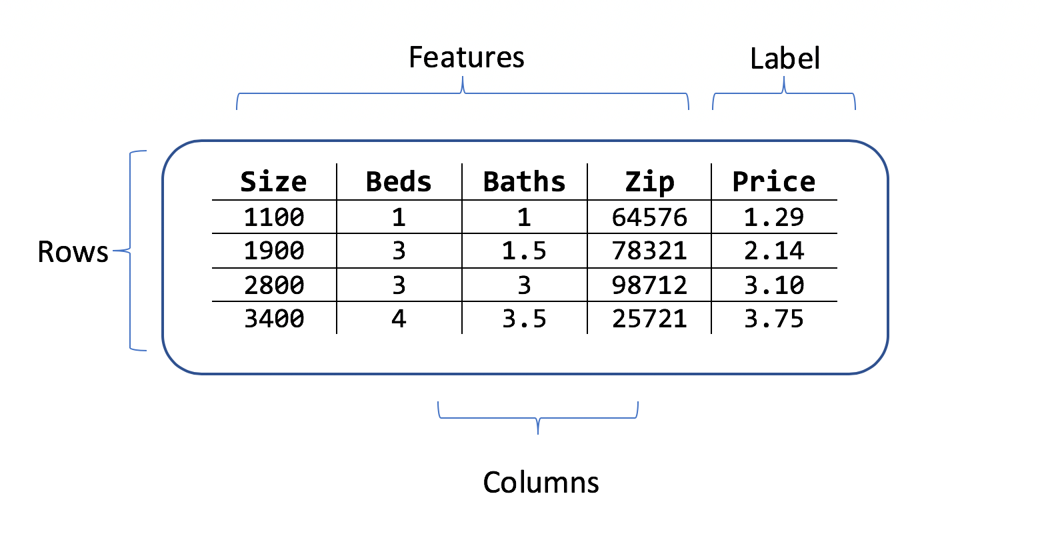
\includegraphics[scale=.3]{../05-pictures/lesson-1-1_pic_6.png} 
\end{center}	
	
\end{frame}
%..................................................................
\begin{frame}{Features and Labels}{Defining Machine Learning}
	\begin{itemize}
		\item For example, when predicting the \textbf{price of a house}, the \textit{features} could be the \textit{square meters of living space}, \textit{the number of bedrooms}, \textit{the number of bathrooms}, \textit{the size of the garage} and so on. 
		\item The \textit{label} would be \textit{the house price};  
	\end{itemize}
\begin{center}
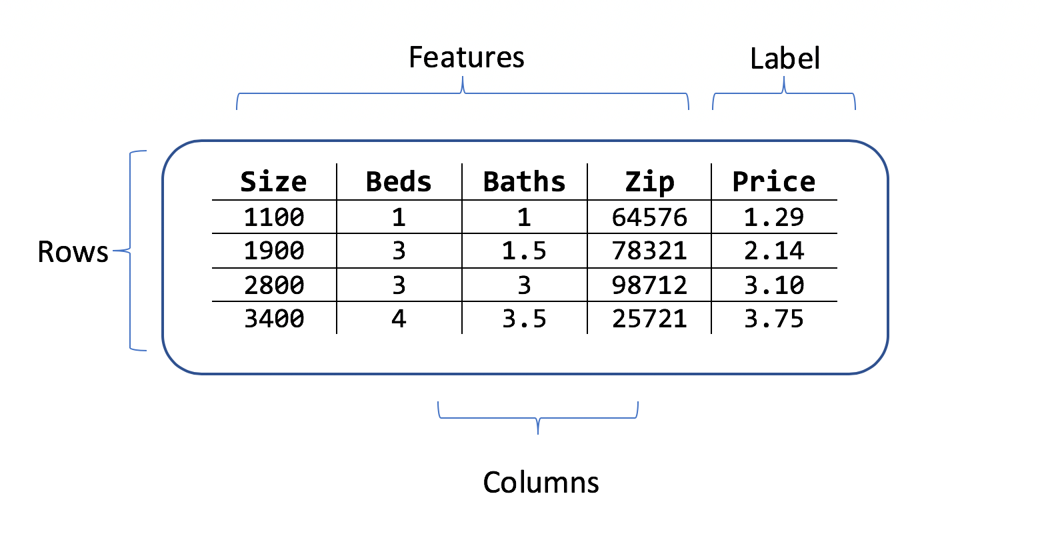
\includegraphics[scale=.35]{../05-pictures/lesson-1-1_pic_7.png} 
\end{center}	
\end{frame}
%__________________________________________________________________________
%
%\subsection{Cost Functions}
%__________________________________________________________________________
%
\begin{frame}{Cost Function}{Defining Machine Learning}
\begin{itemize}
\item In Machine Learning a \textbf{Cost Function} or loss function is used to represent \hly{\text{how far away a mathematical model is from the real data}};
\item One adjust the mathematical model usually by varying parameters within the model so as to \ul{minimize the const function};
\item Let's take for example a very simple model of the form
$$y = \theta_0 + \theta_1 \,x$$
where the $\theta$s are the parameters that we want to find to give us the best fit to the data;
\item Call this function $h_\theta (x)$ to emphasize the dependence on both the variable $x$ and the two parameters $\theta_0$ and $\theta_1$; 
\end{itemize}
\end{frame}
%..................................................................
\begin{frame}{Cost Function}{Defining Machine Learning}
\begin{itemize}
\item We want to measure how far away the data, the $y^{(n)}$s are from the function $h_\theta (x)$;
\item For example in a linear regression problem, a common way to do this is via the quadratic cost function
\begin{equation}\label{cost_function}
		J(\mathbf{\theta}) =  \frac{1}{2N} \sum\limits_{n=1}^N \left[h_\theta \left( x^{(n)} \right) - y ^{(n)}\right]^2 
\end{equation}
\item We wants the parameters that minimize (\ref{cost_function}), almost always you are going to have to do this numerically;
\item If we have a nice convex function then there is a numerical method that will converge to the solution, it is called \textbf{gradient descent}. 
\end{itemize}
\end{frame}
%..................................................................
\begin{frame}{Cost Function}{Defining Machine Learning}
\begin{itemize}
\item The quadratic cost function is probably one of the most used cost function for the regression problem;
\item What if you have a classification problem?
\item There are a lot of different possibilities. For example, for a simple binary classification problem we can use the logistic loss function
\begin{equation}\label{logistic_loss_function}
L(y, \hat{y}) = -[y\log{\hat{y}} + (1 - y)\log{(1 - \hat{y})}]
\end{equation}
\end{itemize}
    \begin{itemize}
        \item $y$ is the true label (0 or 1).
        \item $\hat{y}$ is the predicted probability of class 1.
        \item The function penalizes incorrect predictions more severely.
    \end{itemize}

\end{frame}
%..................................................................
\begin{frame}{Cost Function}{Defining Machine Learning}
\begin{equation}\label{logistic_loss_function}
L(y, \hat{y}) = -[y\log{\hat{y}} + (1 - y)\log{(1 - \hat{y})}]
\end{equation}

    \textbf{When \( y = 1 \)}:
    \[ L(1, \hat{y}) = -\log{\hat{y}} \]
    \begin{itemize}
        \item If \( \hat{y} \) is close to 1, the loss is small.
        \item If \( \hat{y} \) is close to 0, the loss is large.
    \end{itemize}
    \vspace{0.25cm}
    \textbf{When \( y = 0 \)}:
    \[ L(0, \hat{y}) = -\log{(1 - \hat{y})} \]
    \begin{itemize}
        \item If \( \hat{y} \) is close to 0, the loss is small.
        \item If \( \hat{y} \) is close to 1, the loss is large.
    \end{itemize}
\end{frame}
%...................................................................................................
\begin{frame}{Optimization}{Defining Machine Learning}
    \begin{itemize}
        \item Optimization in machine learning refers to the process of adjusting a model’s parameters to minimize (or maximize) a given objective function. 
        \item This function, often called the loss function, measures how well the model's predictions match the actual data. 
        \item The goal is to find the best set of parameters that improve the model’s performance.
    \end{itemize}
\end{frame}
%...................................................................................................
\begin{frame}{Optimization}{Defining Machine Learning}
   \begin{itemize}
      \item   				  						  
		Gradient Descent is a very generic optimization algorithm capable of finding optimal solutions to a wide range of problems. 
	  \item Gradient Descent Algorithm measures the local gradient of the error function with regards to the parameter vector $\theta$, and it goes in the direction of descending gradient. 
	  \item Once the gradient is zero, you have reached a minimum!
      \item Concretely, you start by filling $\theta$ with random values (this is called random initialization), and then you improve it gradually, taking one step at a time, each step attempting to decrease the cost function (e.g., the MSE), until the algorithm converges to a minimum		  
   \end{itemize}
\end{frame}
%...................................................................................................
\begin{frame}{Optimization}{Defining Machine Learning}
An important parameter in Gradient Descent is the size of the steps, determined by
the learning rate hyperparameter. 
   \begin{center}
   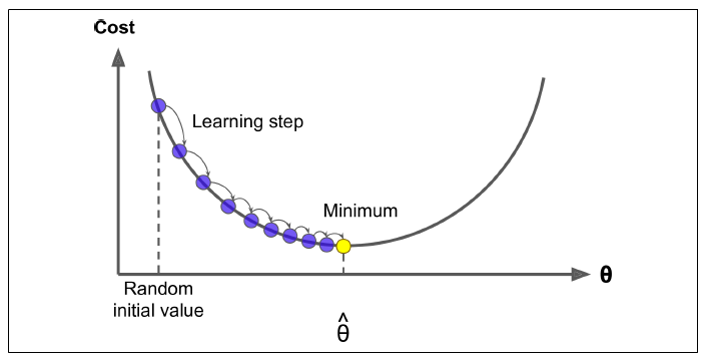
\includegraphics[scale=.6]{../05-pictures/lesson-1-1_pic_8.png} 	
   \end{center}
\end{frame}
%...................................................................................................
\begin{frame}{Optimization}{Defining Machine Learning}
If the learning rate is too small, then the algorithm
will have to go through many iterations to converge, which will take a long time...   \begin{center}
   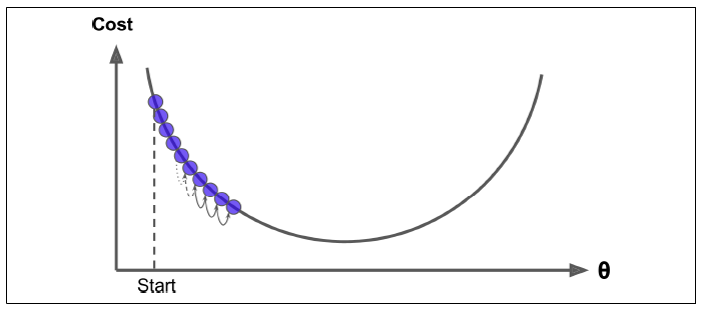
\includegraphics[scale=.6]{../05-pictures/lesson-1-1_pic_9.png} 	
   \end{center}
\end{frame}
%...................................................................................................
\begin{frame}{Optimization}{Defining Machine Learning}
... on the other hand, if the learning rate is too high, you might jump across the valley. This might make the algorithm diverge failing to find a good solution. 
   \begin{center}
   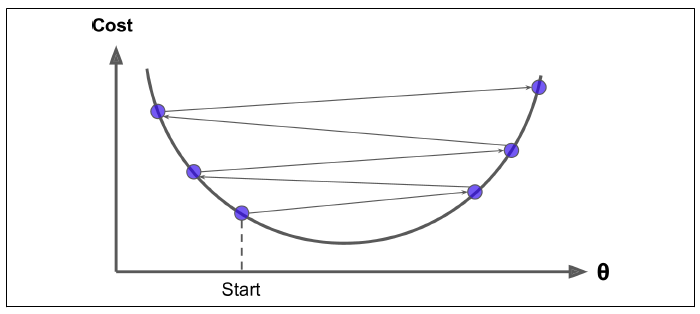
\includegraphics[scale=.6]{../05-pictures/lesson-1-1_pic_10.png} 	
   \end{center}
\end{frame}
%...................................................................................................
\begin{frame}{Optimization}{Defining Machine Learning}
Having defined an appropriate learning rate, the scheme works as follow
\begin{itemize}
\item Start with an initial guess for each parameter $\theta_k$;
\item Move $\theta_k$ in the direction of the slope

\begin{empheq}[box=\tcbhighmath]{align*}
\text{New}\: \theta_k = \text{Old}\: \theta_k - \beta \frac{\partial J}{\partial \theta_k}
\end{empheq}

where $\beta$ is our learning rate;
\end{itemize}
\begin{tcolorbox}
In the above description of gradient descent we have used all of the data points simultaneously. This is called \textbf{batch gradient descent}
\end{tcolorbox}
\end{frame}
%===================================================================================================
\section{The Machine Learning Process
\\ \scalebox{0.8}{General Workflow of a ML Application}}
%..................................................................
\begin{frame}{The Machine Learning Process}
The development and deployment of ML models follow a structured, multi-step process:

	\begin{center}
	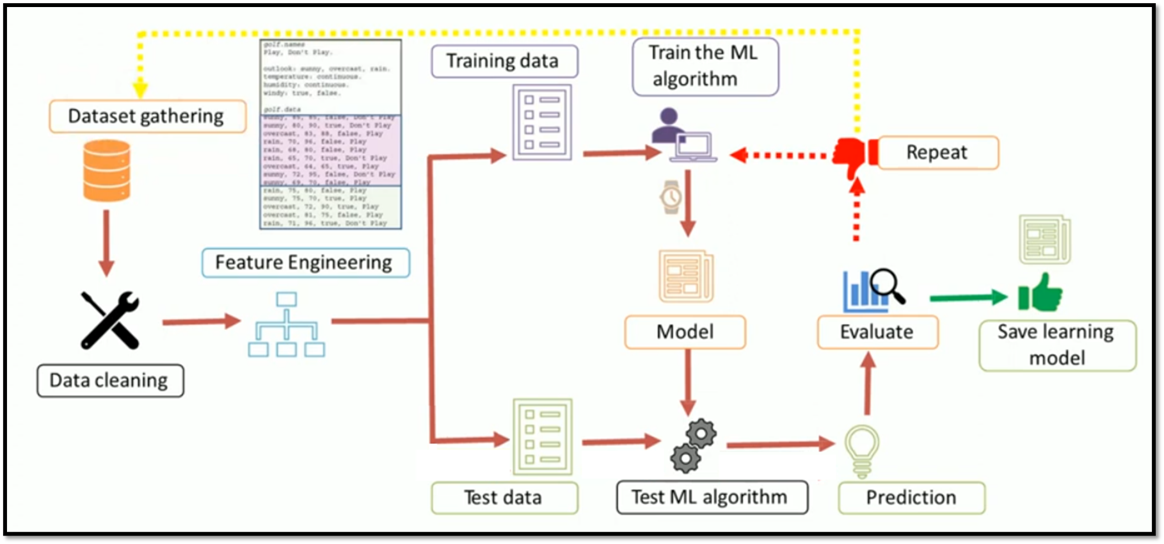
\includegraphics[scale=0.4]{../05-pictures/lesson-1-1_pic_11.png}
	\end{center}
\end{frame}
%..................................................................
\begin{frame}{The Machine Learning Process}
The development and deployment of ML models follow a structured, multi-step process:

	\begin{center}
	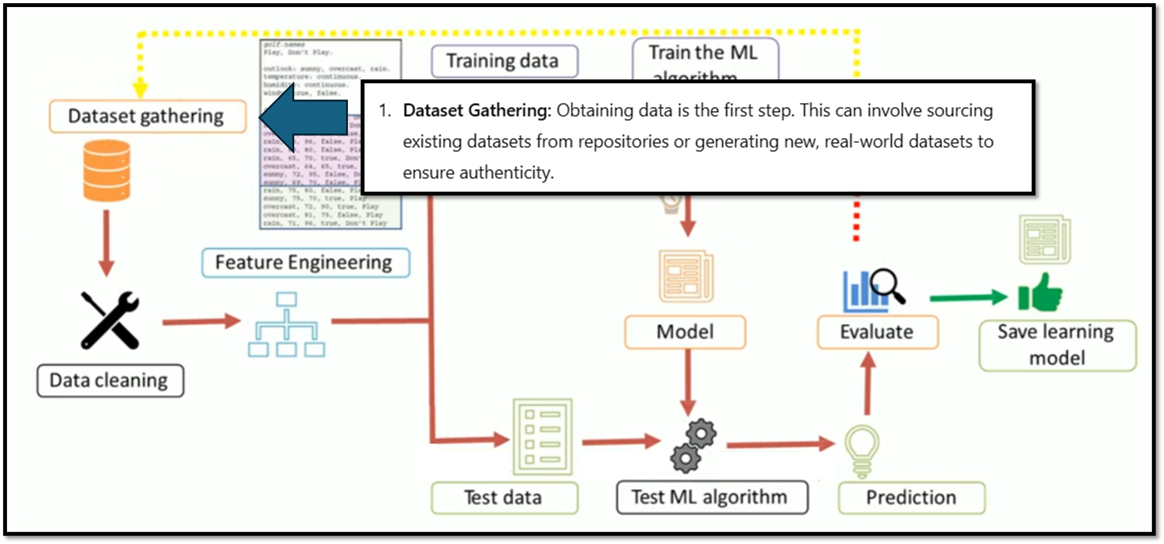
\includegraphics[scale=0.4]{../05-pictures/lesson-1-1_pic_12.png}
	\end{center}
\end{frame}
%..................................................................
\begin{frame}{The Machine Learning Process}
The development and deployment of ML models follow a structured, multi-step process:

	\begin{center}
	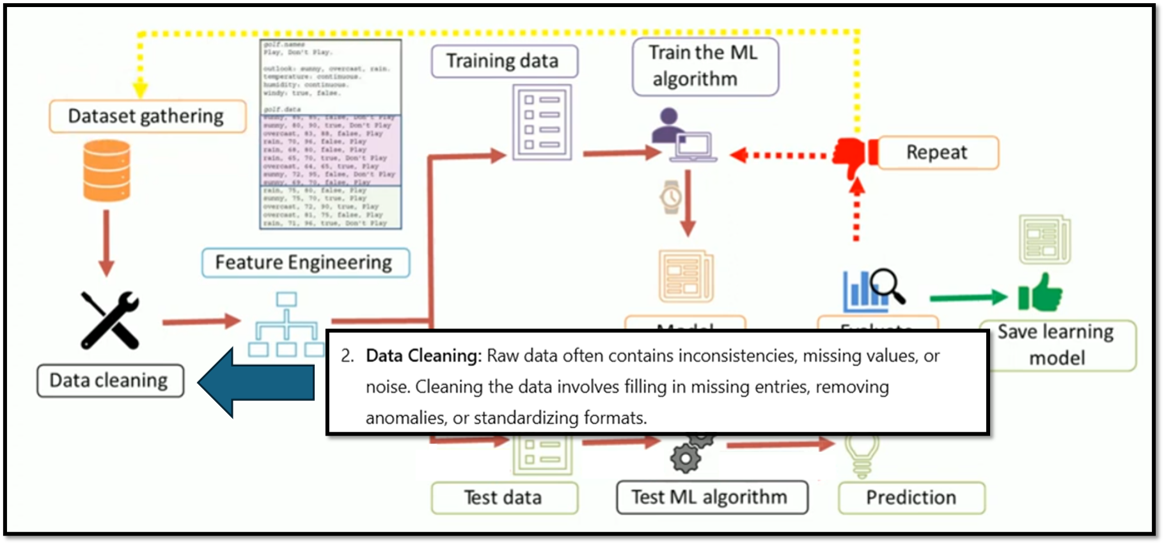
\includegraphics[scale=0.4]{../05-pictures/lesson-1-1_pic_13.png}
	\end{center}
\end{frame}
%..................................................................
\begin{frame}{The Machine Learning Process}
The development and deployment of ML models follow a structured, multi-step process:

	\begin{center}
	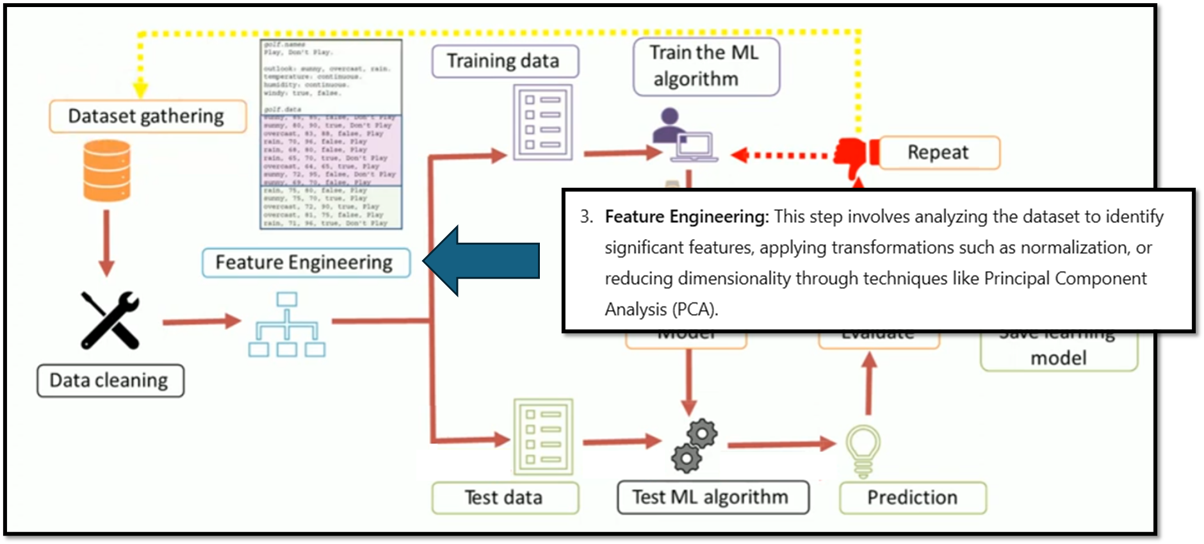
\includegraphics[scale=0.39]{../05-pictures/lesson-1-1_pic_14.png}
	\end{center}
\end{frame}
%..................................................................
\begin{frame}{The Machine Learning Process}
The development and deployment of ML models follow a structured, multi-step process:

	\begin{center}
	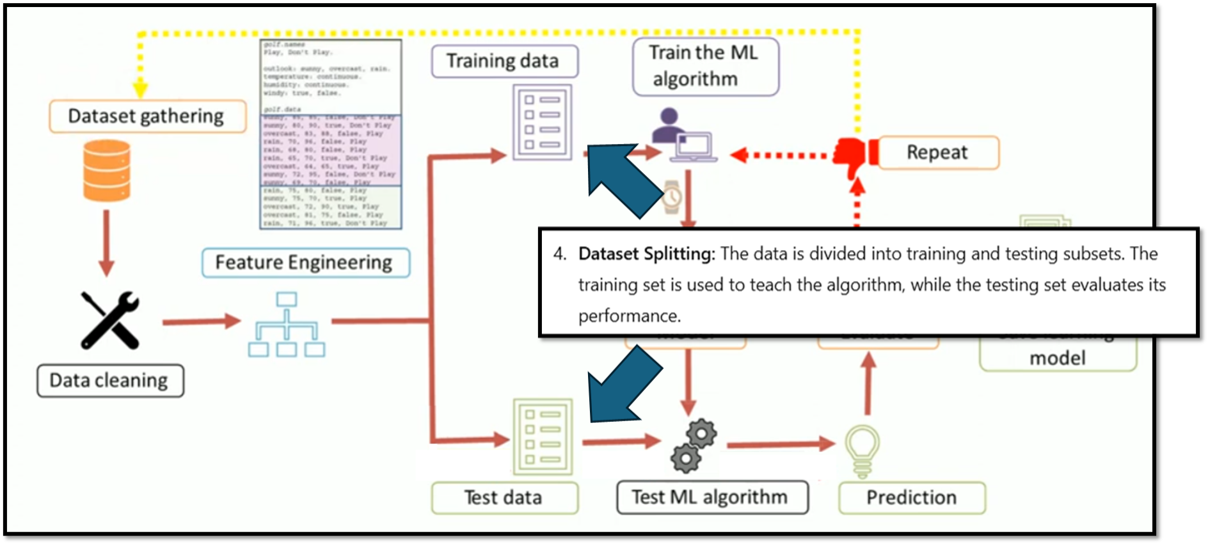
\includegraphics[scale=0.39]{../05-pictures/lesson-1-1_pic_15.png}
	\end{center}
\end{frame}
%..................................................................
\begin{frame}{The Machine Learning Process}
The development and deployment of ML models follow a structured, multi-step process:

	\begin{center}
	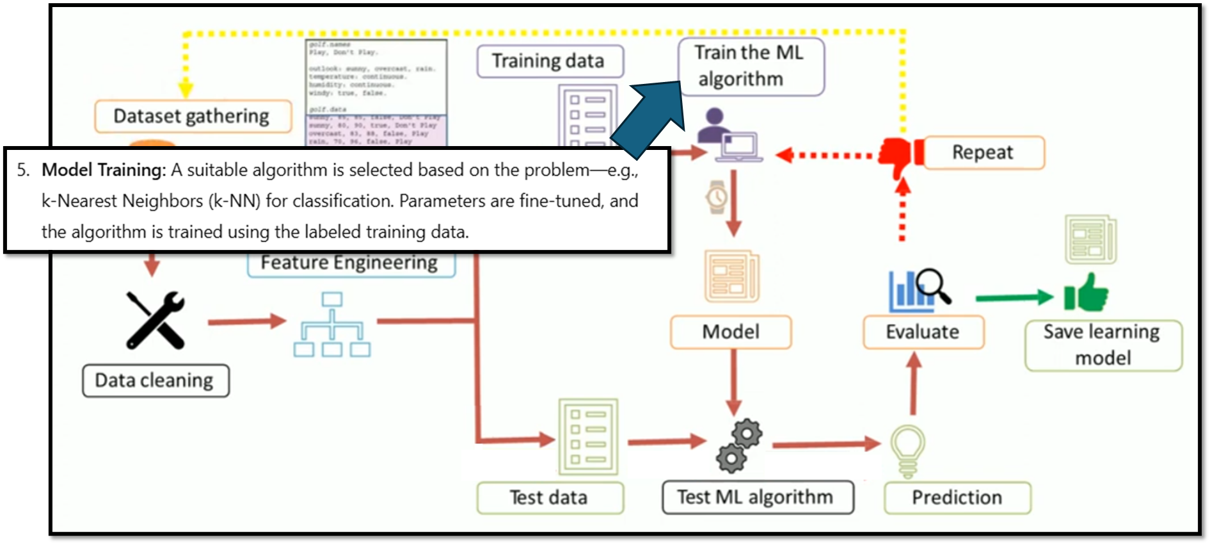
\includegraphics[scale=0.38]{../05-pictures/lesson-1-1_pic_16.png}
	\end{center}
\end{frame}
%..................................................................
\begin{frame}{The Machine Learning Process}
The development and deployment of ML models follow a structured, multi-step process:

	\begin{center}
	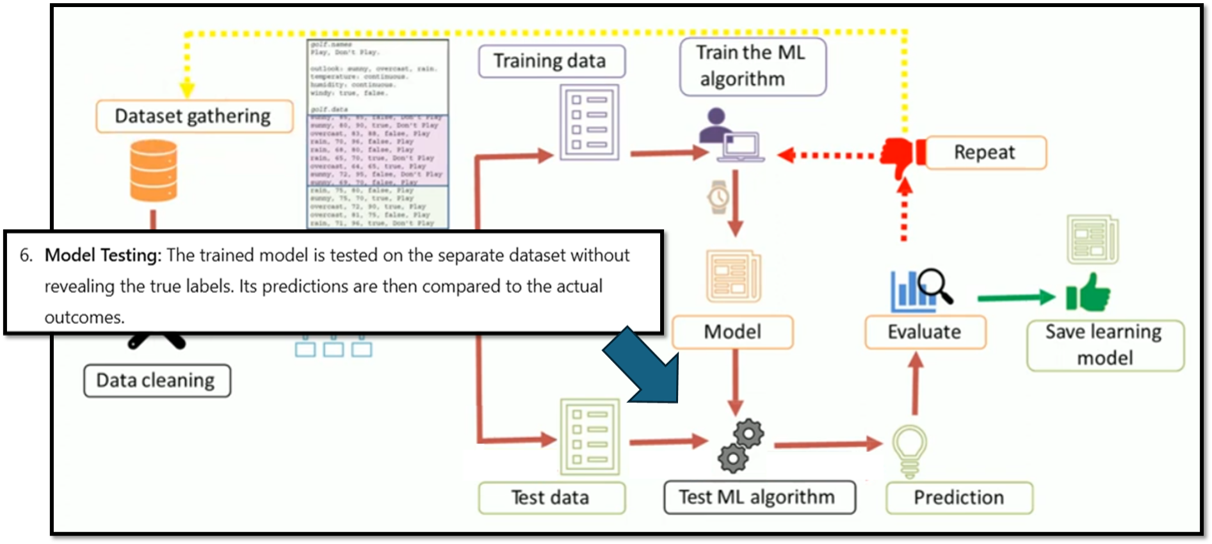
\includegraphics[scale=0.38]{../05-pictures/lesson-1-1_pic_17.png}
	\end{center}
\end{frame}
%..................................................................
\begin{frame}{The Machine Learning Process}
The development and deployment of ML models follow a structured, multi-step process:

	\begin{center}
	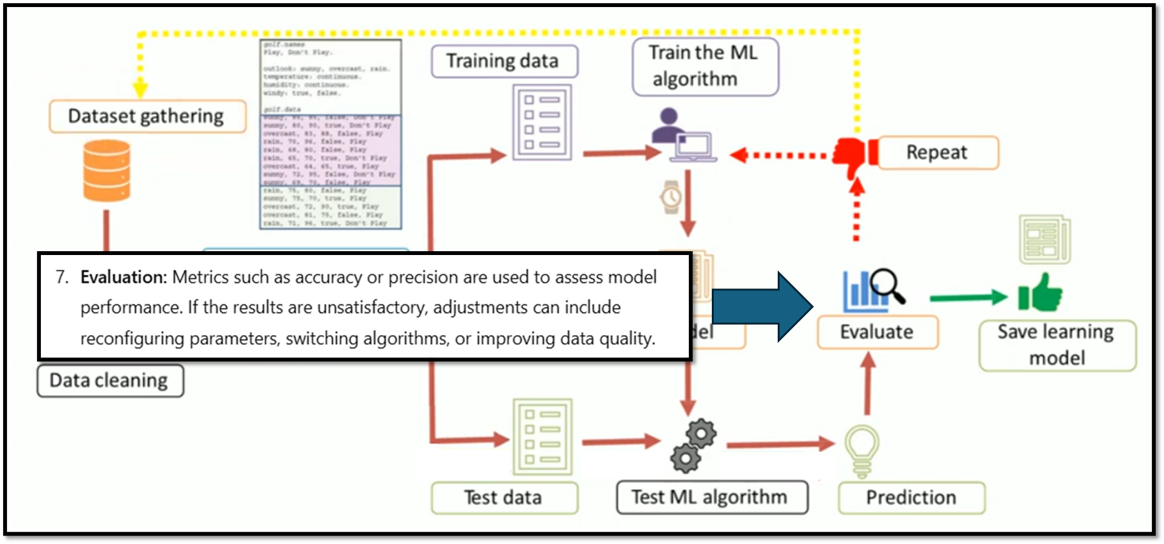
\includegraphics[scale=0.4]{../05-pictures/lesson-1-1_pic_18.png}
	\end{center}
\end{frame}
%===================================================================================================
\section{Types of Machine Learning Models}
%..................................................................
\begin{frame}{Types of Machine Learning}
ML algorithms can be broadly categorized into four types:

	\begin{center}
	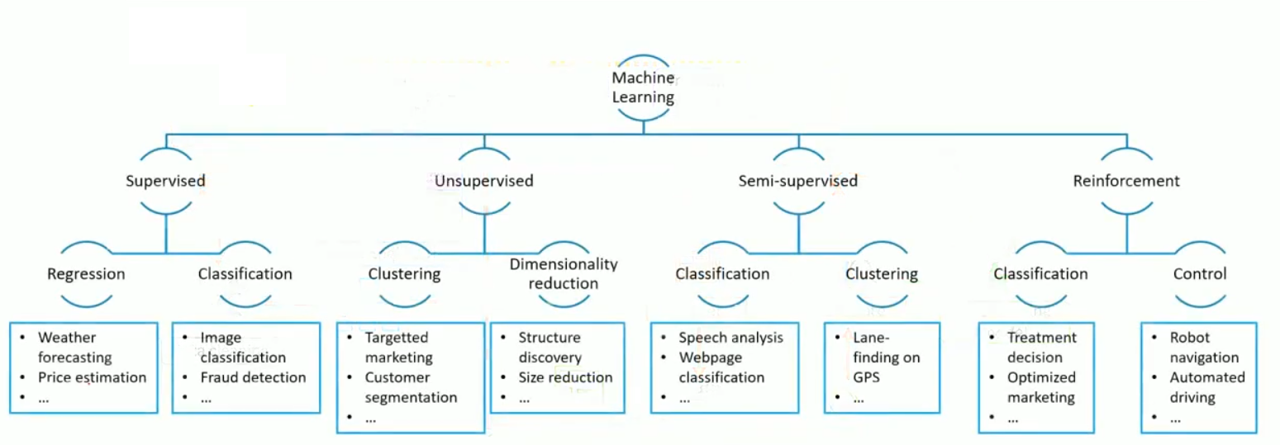
\includegraphics[scale=0.35]{../05-pictures/lesson-1-1_pic_19.png}
	\end{center}
\end{frame}
%..................................................................
\begin{frame}{Supervised Learning}{Types of Machine Learning}
\textbf{Supervised Learning}

	\begin{itemize}
		\item In supervised learning, the algorithm is trained on labeled data, meaning both input variables (features) and corresponding output variables (labels) are provided. 

		\item The goal is to learn the mapping between inputs and outputs. 

	\end{itemize}


Supervised learning includes:

	\begin{itemize}
		\item \textbf {Regression}: Predicting continuous numerical values, such as temperatures or stock prices.

		\item \textbf {Classification}: Categorizing data into discrete groups, such as identifying whether an email is spam or not.

	\end{itemize}
\end{frame}
%..................................................................
\begin{frame}{Supervised Learning}{Types of Machine Learning}
	\begin{center}
	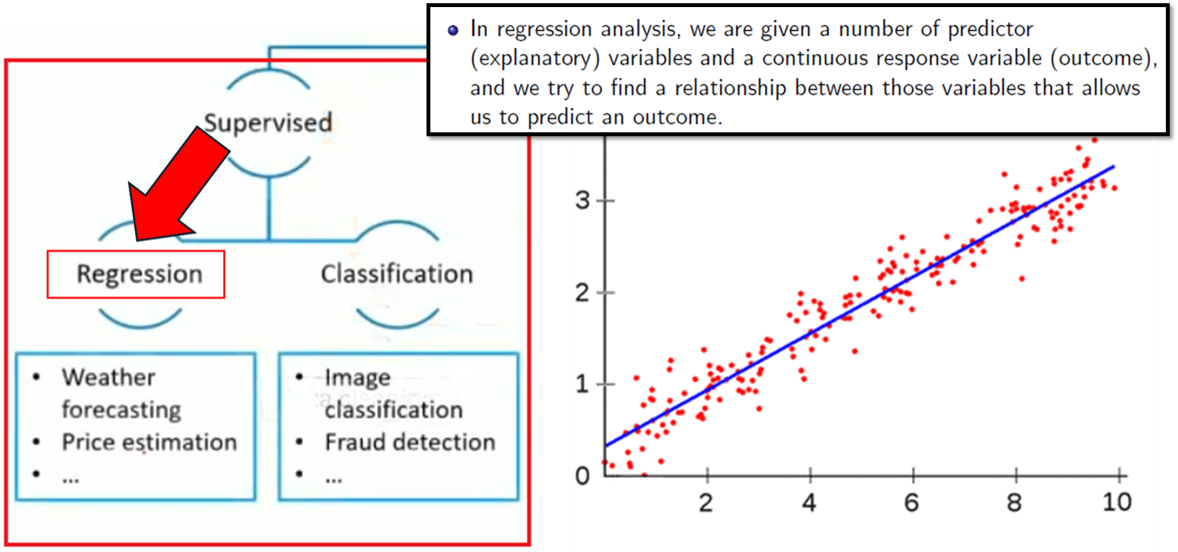
\includegraphics[scale=0.38]{../05-pictures/lesson-1-1_pic_20.png}
	\end{center}
\end{frame}
%..................................................................
\begin{frame}{Supervised Learning}{Types of Machine Learning}
	\begin{center}
	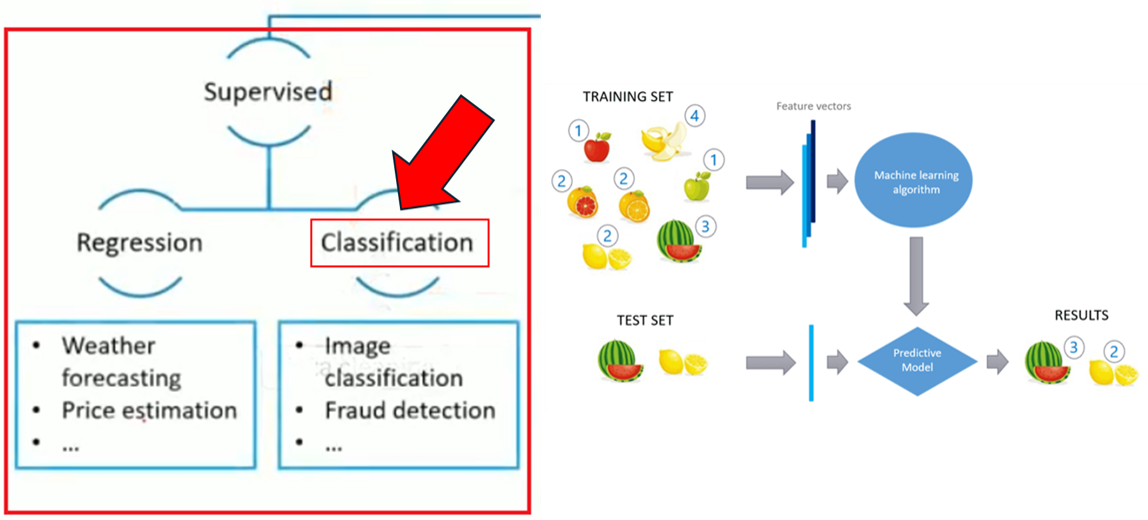
\includegraphics[scale=0.38]{../05-pictures/lesson-1-1_pic_21.png}
	\end{center}
\end{frame}
%..................................................................
\begin{frame}{Supervised Learning}{Types of Machine Learning }
\begin{itemize}
\item From a formal poin of view, supervised learning process involves input variables, which we call $X$, and an output variable, which we call $Y$. 

\item We use an algorithm \hly{\text{to learn the mapping function}} from the input to the output. 

\item In simple mathematics, the output $Y$ is a dependent variable of input $X$ as illustrated by:

$$Y = f(X)$$
\end{itemize}

\begin{tcolorbox}
Here, our end goal is to try to \textbf{approximate the mapping function} $f$, so that we can \textbf{predict} the output variables $Y$ when we have new input data $X$.
\end{tcolorbox}
\end{frame}
%..................................................................
\begin{frame}{Unsupervised Learning}{Types of Machine Learning}
\textbf{Unsupervised Learning}
	\begin{itemize}
		\item Unsupervised learning involves analyzing data without labeled outputs. 

		\item The algorithm identifies hidden patterns or structures. 

	\end{itemize}
Two primary uses include:

	\begin{itemize}
		\item \textbf{Clustering}: Grouping similar data points, for instance, segmenting customers for targeted marketing.

		\item \textbf{Dimensionality Reduction}: Simplifying datasets by reducing features while preserving essential information, often used to speed up computations or eliminate noise.
	\end{itemize}
\end{frame}
%..................................................................
\begin{frame}{Unsupervised Learning}{Types of Machine Learning}
\begin{itemize}
\item Unsupervised algorithms attempt to find some sort of underlying structure in the data. 

\item Are some observations clustered into groups? Are there interesting relationships between different features? Which features carry most of the information?
\end{itemize}
\begin{center}
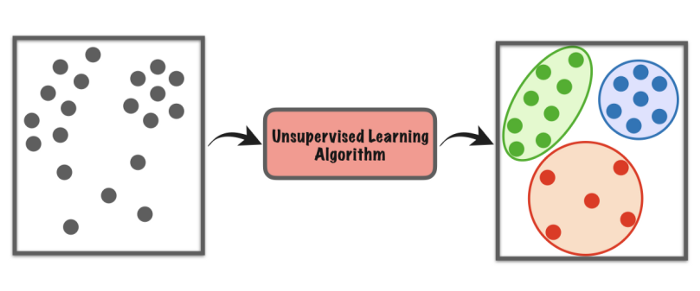
\includegraphics[scale=.35]{../05-pictures/lesson-1-1_pic_22.png} 
\end{center}
\end{frame}
%..................................................................
\begin{frame}{Unsupervised Learning}{Types of Machine Learning}
	\begin{itemize}
		\item The data for \textbf{Unsupervised Learning} consists of features but no labels because the model is being used to identify patterns not to forecast something. 
		\item For example we could use an unsupervised model to classify the houses that exist in a certain neghborhood without trying to predict any price.
	\end{itemize}
\begin{center}
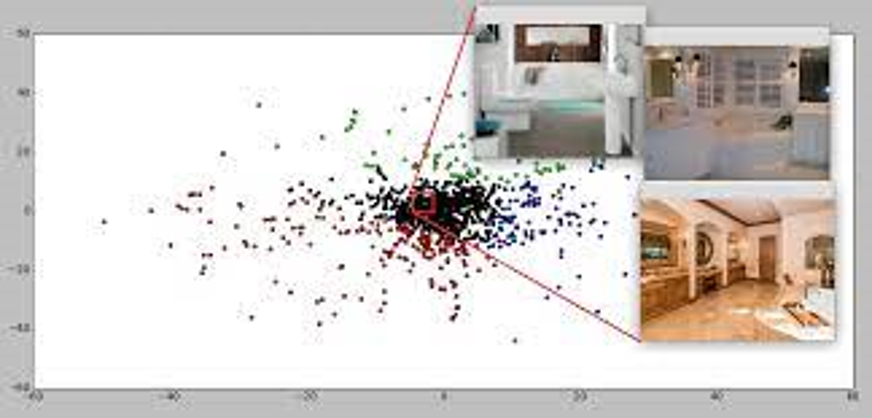
\includegraphics[scale=.35]{../05-pictures/lesson-1-1_pic_23.png} 
\end{center}	
\end{frame}
%..................................................................
\begin{frame}{Semi-Supervised Learning}{Types of Machine Learning}
\textbf{Semi-Supervised Learning}

	\begin{itemize}
		\item Semi-supervised learning combines elements of supervised and unsupervised methods. 

		\item It operates on datasets where only some entries are labeled. Techniques may include assigning labels to unlabeled data or training the model iteratively on both labeled and unlabeled subsets. 

		\item Applications include speech analysis and web page classification.

	\end{itemize}
\end{frame}
%..................................................................
\begin{frame}{Reinforcement Learning}{Types of Machine Learning}
\textbf{Reinforcement Learning}

	\begin{itemize}
		\item Reinforcement learning involves algorithms that learn through interaction with their environment. 

		\item These models improve by receiving rewards or penalties for their actions, refining their strategies over time. 

		\item Applications range from training autonomous vehicles to optimizing marketing strategies. 
	\end{itemize}
\end{frame}
%===================================================================================================
\section{Learning Tools}
%===================================================================================================
%______________________________________________________________________________
%
\subsection{Python and Anaconda}
%______________________________________________________________________________
%
%..................................................................
\begin{frame}{Python and Anaconda}
	\begin{itemize}
		\item Python is one of the most popular programming languages for data science and thanks to its very active developer and open source community, a large number of
useful libraries for scientific computing and machine learning have been developed.
\item Although the performance of interpreted languages, such as Python, for
computation-intensive tasks is inferior to lower-level programming languages,
extension libraries such as \textbf{NumPy}, \textbf{Matplotlib} and \textbf{Pandas}, among the others, have been developed that build
upon lower-layer Fortran and C implementations for fast vectorized operations
on multidimensional arrays.
	\end{itemize}
\end{frame}
%..................................................................
\begin{frame}{Python and Anaconda}
	\begin{itemize}
		\item For machine learning programming tasks, we will mostly refer to the \textbf{scikit-learn}
library, which is currently one of the most popular and accessible open source
machine learning libraries. 
\item In the last part of these lessons, when we focus on a subfield
of machine learning called deep learning, we will use the latest version of the
\textbf{Keras} library, which specializes in training so-called deep neural network
models very efficiently.  
 
	\end{itemize}
\end{frame}


%...................................................................................................
\begin{frame}{Installing Python and Anaconda}
\footnotesize{
\begin{itemize}
\item  To download an Anaconda distribution, you can use the official download page: \textbf{https://www.anaconda.com/download/}
\item Here, you can select your platform and then choose the installer. For this, you can choose which version you want and whether 32-bit or 64-bit.
\end{itemize}}
\normalsize
\begin{center}
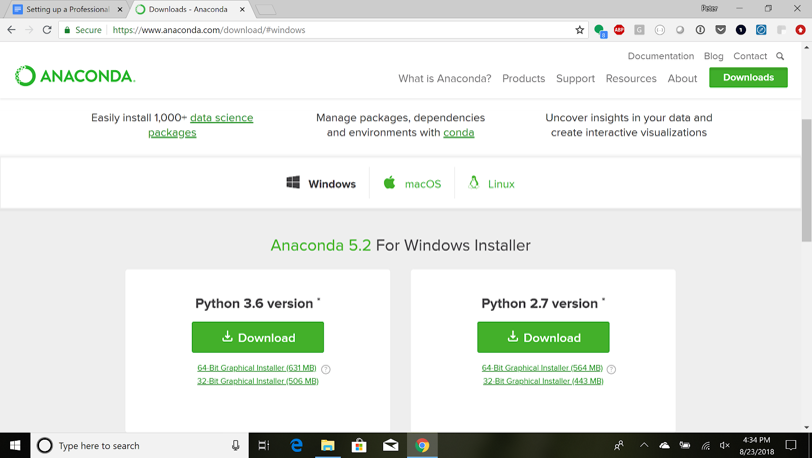
\includegraphics[scale=.4]{../05-pictures/lesson-1-1_pic_24.png} 
\end{center}
\end{frame}
%...................................................................................................
\begin{frame}{Testing Your Installation}
To test your installation, on Windows, click on Start and then Anaconda Navigator in the program list (or search for Anaconda in the search bar and select Anaconda Navigator). On a Mac, open up the finder, and in the Applications folder, double click on Anaconda-Navigator.
\begin{center}
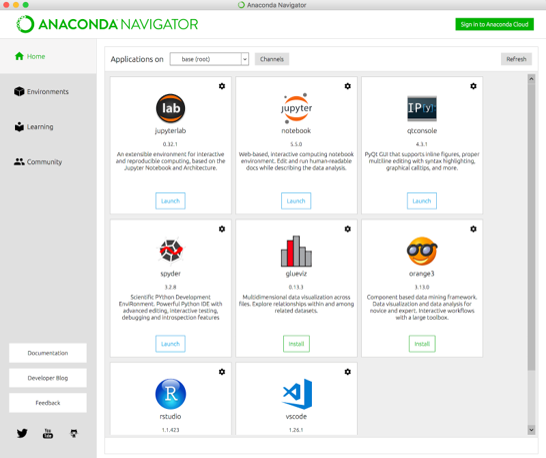
\includegraphics[scale=.4]{../05-pictures/lesson-1-1_pic_25.png} 
\end{center}
\end{frame}
%______________________________________________________________________________
%
%\subsection{Package Managers}
%______________________________________________________________________________
%
\begin{frame}{Package Managers}
\begin{itemize}
\item  Anaconda will give you two package managers- pip and conda. 

\item When some packages aren’t available with conda, you can use pip to install them. 

\item Note that using pip to install packages also available to conda may cause an installation error.

\item After we have successfully installed Python, we can execute pip from the terminal to install additional Python packages:
\begin{center}
\textbf{pip install SomePackage}
\end{center}

\item Already installed packages can be updated via the --upgrade flag:
\begin{center}
\textbf{pip install SomePackage --upgrade}
\end{center}

\end{itemize}
\end{frame}
%______________________________________________________________________________
%
\subsection{Jupyter Notebook}
%______________________________________________________________________________
%
\begin{frame}{Teaching tools: Jupyter Notebook}
\begin{itemize}
\item The Python world developed the IPython notebook system. 
\item Notebooks  allow you to write text, but you insert code blocks as "cells" into the notebook. 
\item A notebook is interactive, so you can execute the code in the cell directly!
\item Recently the Notebook idea took a much enhanced vision and scope, to explicitly allow languages other than Python to run inside the cells. 
\item Thus the Jupyter Notebook was born, a project initially aimed at Julia, Python and R (Ju-Pyt-e-R). But in reality many other languages are supported in Jupyter.
\end{itemize}
\end{frame}
%...................................................................................................
\begin{frame}{Teaching tools: Jupyter Notebook}
\begin{columns}[T] % align columns
\begin{column}{.48\textwidth}
		\begin{itemize}
			\item Jupyter was designed to enable sharing of notebooks with other people. 
			\item The idea is that you can write some code, mix some text with the code, and publish this as a notebook.  
\item In the notebook they can see the code as well as the actual results of running the code.
		\end{itemize}
\end{column}%
\hfill%
\begin{column}{.48\textwidth}
	%\fbox{
		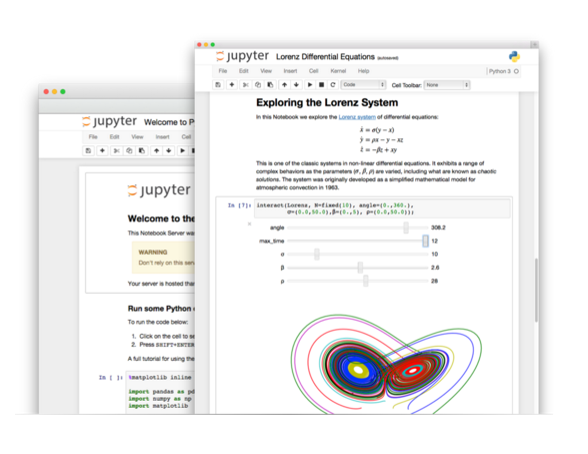
\includegraphics[width=\linewidth]{../05-pictures/lesson-1-1_pic_26.PNG}
	%}
\end{column}%
\end{columns}
\end{frame}
%...................................................................................................
\begin{frame}{Teaching tools: Jupyter Notebook}
\begin{columns}[T] % align columns
\begin{column}{.48\textwidth}
		\begin{itemize}
\item This is a nice way of sharing little experimental snippets, but also to publish more detailed reports with explanations and full code sets.  
\item Of course, a variety of web services allows you to post just code snippets (e.g. gist). 
\item What makes Jupyter different is that the service will actually render the code output.
		\end{itemize}
\end{column}%
\hfill%
\begin{column}{.48\textwidth}
	%\fbox{
		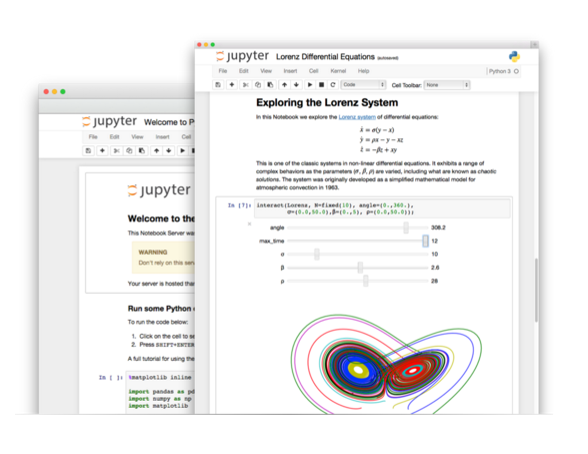
\includegraphics[width=\linewidth]{../05-pictures/lesson-1-1_pic_27.PNG}
	%}
\end{column}%
\end{columns}
\end{frame}
%...................................................................................................
\begin{frame}{Teaching tools: Jupyter Notebook}
\begin{itemize}
\item  As we saw earlier, the Jupyter Notebook ships with Anaconda. To run it, you can get in your virtual environment and type the following command: \textbf{jupyter notebook};
\item Or directly from the Windows Menu...
\begin{center}
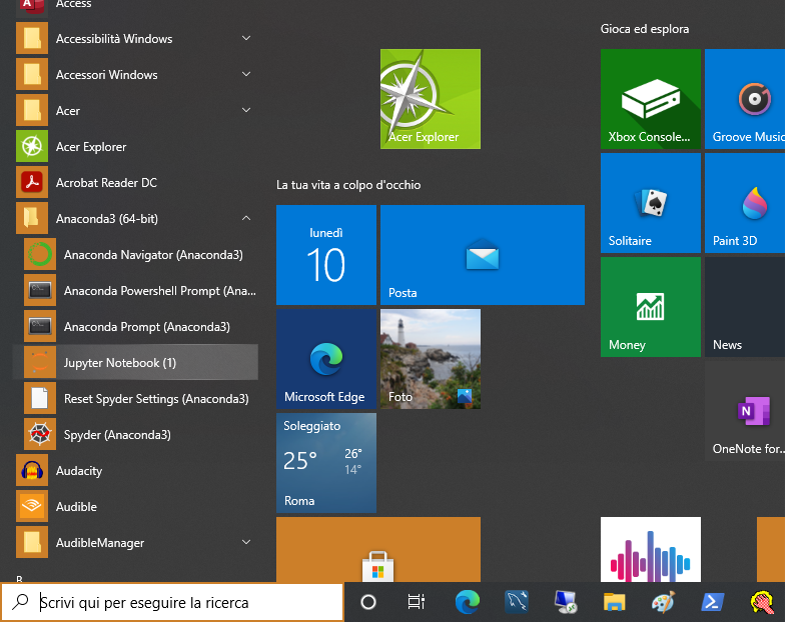
\includegraphics[scale=.3]{../05-pictures/lesson-1-1_pic_28.PNG} 
\end{center}
\end{itemize}
\end{frame}
%...................................................................................................
\begin{frame}{Teaching tools: Jupyter Notebook}
\begin{itemize}
\item You can find this at \textbf{http://localhost:8888/tree}
\item Now to run Python here, you can create a new file. 
\begin{center}
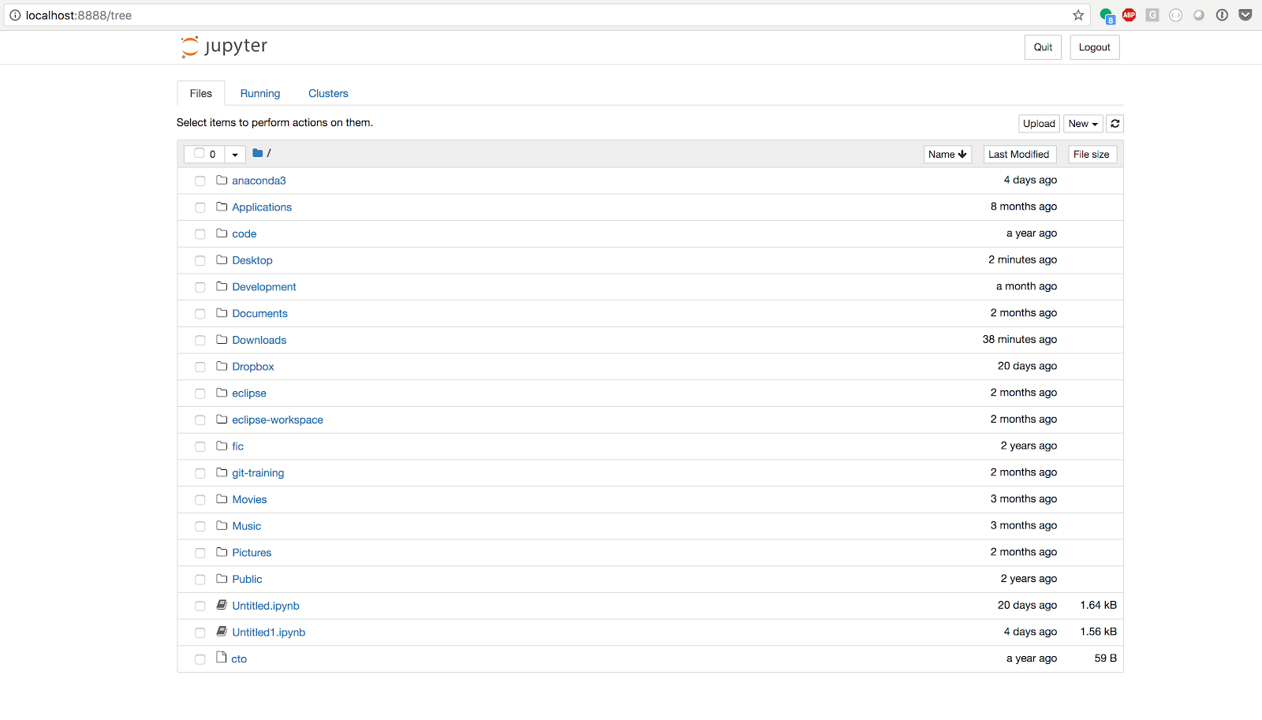
\includegraphics[scale=.175]{../05-pictures/lesson-1-1_pic_29.PNG} 
\end{center}
\end{itemize}
\end{frame}
%...................................................................................................
\begin{frame}{Teaching tools: Jupyter Notebook}

To make sure it’s working, click in the cell and type the following:

\begin{center}
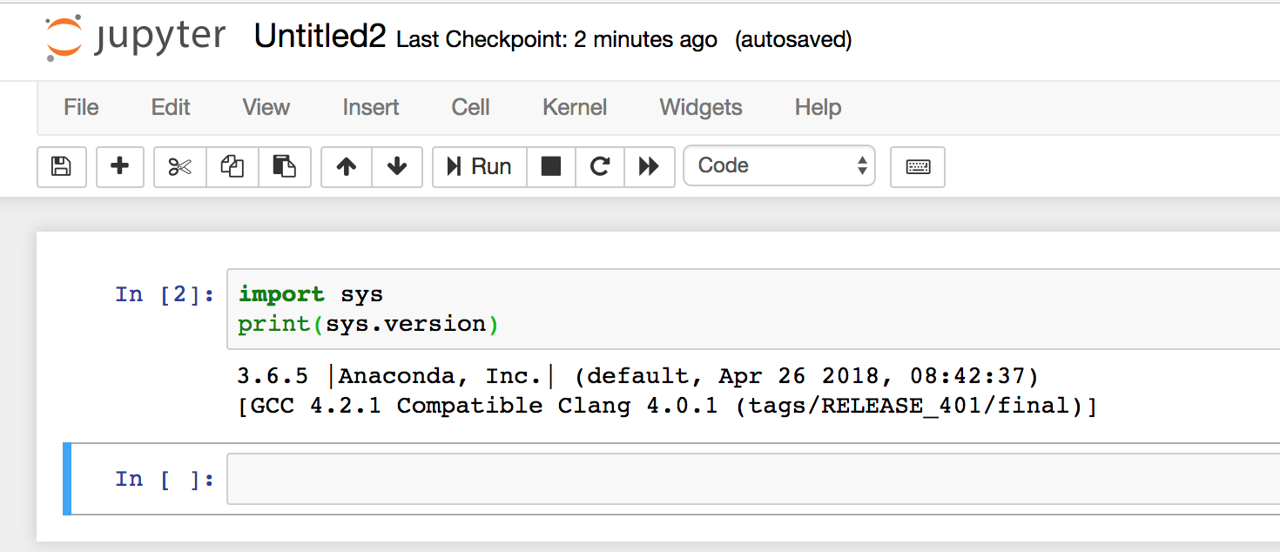
\includegraphics[scale=.175]{../05-pictures/lesson-1-1_pic_30.PNG} 
\end{center}
\end{frame}
%______________________________________________________________________________
%
\subsection{Google Colab}
%______________________________________________________________________________
%
\begin{frame}{Teaching tools: Google Colab}
	\noindent\begin{minipage}{0.5\textwidth}
		
\includegraphics[width=\linewidth]{../05-pictures/lesson-1-1_pic_31.PNG}
	\end{minipage}%
	\hfill%
	\begin{minipage}{0.5\textwidth}
		\begin{itemize}
			\item Colaboratory, or "Colab" for short, is a product from Google Research. \item Colab allows anybody to write and execute arbitrary python code through the browser, and is especially well suited to machine learning, data analysis and education. 
		\end{itemize}
	\end{minipage}
\vfill
\footnotesize{\textbf{https://colab.research.google.com/notebooks/intro.ipynb?hl=en}}
\end{frame}
%...................................................................................................
\begin{frame}{Teaching tools: Google Colab}
	\noindent\begin{minipage}{0.5\textwidth}
		
\includegraphics[width=\linewidth]{../05-pictures/lesson-1-1_pic_32.PNG}
	\end{minipage}%
	\hfill%
	\begin{minipage}{0.5\textwidth}
		\begin{itemize}
\item More technically, Colab is a hosted Jupyter notebook service that requires no setup to use, while providing free access to computing resources including GPUs.
\item Colab notebooks are stored in \textit{Google Drive}, or can be loaded from \textit{GitHub}. Colab notebooks can be shared just as you would with Google Docs or Sheets.
		\end{itemize}
	\end{minipage}
\vfill	
\footnotesize{\textbf{https://colab.research.google.com/notebooks/intro.ipynb?hl=en}}
\end{frame}


\end{document}
